%# -*- coding: utf-8 -*-
% !TEX encoding = UTF-8 Unicode
\RequirePackage{fixltx2e}
\documentclass[aps,pre,12pt,preprint,onecolumn,showpacs,showkeys,UTF8]{revtex4-1}
\usepackage{ctex}
\usepackage{mathrsfs}
\usepackage{setspace,dcolumn}
\usepackage{subfigure}
\usepackage{graphicx,psfrag,epsfig}
\usepackage[font=small,format=plain,labelfont=bf,textfont=it,justification=raggedright,singlelinecheck=false]{caption}
\usepackage{amsmath,amsfonts,amssymb,amsthm,bm,upgreek}
\usepackage{geometry}
\usepackage[mathscr]{eucal}
\usepackage{titlesec}
\usepackage{tabularx}
\titleformat{\section}{\bf\fangsong\zihao{4}}{\thesection}{0.75em}{}
\geometry{top=2.54cm,bottom=2.54cm,left=3cm,right=3cm}
\renewcommand\appendixname{附录}
\renewcommand\abstractname{}%摘要
\renewcommand\tablename{表}
\renewcommand\figurename{图}
\makeatletter
\def\@keys@name{\songti\zihao{-4}{\bf 关键词:}}
\def\Received@name{\zihao{-5}{接收} }
\def\Revised@name{\zihao{-5}{修订} }
\def\Accepted@name{\zihao{-5}{采纳} }
\def\Published@name{\zihao{-4}{发表} }
\makeatother
\linespread{1.6}
\renewcommand{\labelenumi}{\alph{enumi}.}
\leftmargini=20mm

\begin{document}

\title{\bf\heiti\zihao{3}非线性晶体中的二倍频特性研究\vspace{15mm}}
\author{\fangsong 乔颢\vspace{2mm}}
\affiliation{\songti\zihao{-4}北京大学物理学院2011级2班~~~~学号:1100011354 \vspace{2mm}}
\keywords{半导体激光器,非线性晶体,二倍频,转换效率}
\email{1993422qsh@gmail.com; 18600200672}
\begin{abstract}
	\vspace{10mm}
	\begin{spacing}{1.5}
		\songti\zihao{-4}
		本实验利用半导体激光器作为泵浦光源,使用Nd:YAG和Nd:YVO$_4$晶体作为激光晶体,产生了1064nm的红外激光器。两者最大转换效率约为40\%。同时探究了Cr$^{4+}$:YAG晶体被动调Q产生的激光脉冲随着泵浦电流变大,脉冲频率变高的性质,以及使用KTP晶体产生二倍频的532nm绿色激光,探究了其倍频后输出功率和未倍频输出功率的相关关系。
	\end{spacing}
\end{abstract}

\maketitle

\section{引言}
半导体泵浦固体激光器是以激光二极管代替闪光灯泵浦固体激光器介质的固体激光器,具有效率高、体积小、寿命长等一系列优点。上世纪80年代起,生长半导体激光器技术得到了蓬勃的发展,使得其功率和效率都有了极大的提高,也大大促进了泵浦固体激光器的发展。其效率提高,体积减少。随着激光技术的发展非线性光学也得以蓬勃的发展。与线性光学不同的是,物质的许多光学参数随着如射光变化。于是产生了很多的新的光学现象。比如说二倍频,三倍频,和频和差频等等。这些作用大大扩展了可获取的激光波长范围,填补了某些波长的空白,并广泛应用到了科学研究、军事、工业、农业、医学等等。

本实验通过半导体激光器产生泵浦光源,利用Nd:YAG晶体和Nd:YVO$_4$晶体产生频率为1064nm激光,探究了激光功率和腔长的关系等。通过此试验,能对非线性光学的基本原理有所理解,掌握了二倍频,和频的产生原理和方法,分析了影响倍频转换效率的主要原因,认识相位匹配在非线性光学过程的重要过程。

\section{实验装置和原理}
本实验用到的装置有泵浦激光源,Nd:YAG激光晶体,Nd:YVO$_4$激光晶体。激光耦合系统,输出腔镜,准之激光器,功率计,调Q晶体以及KTP晶体。实验装置图片如图\ref{g:1}所示:
\begin{figure}[h]
	\begin{center}
		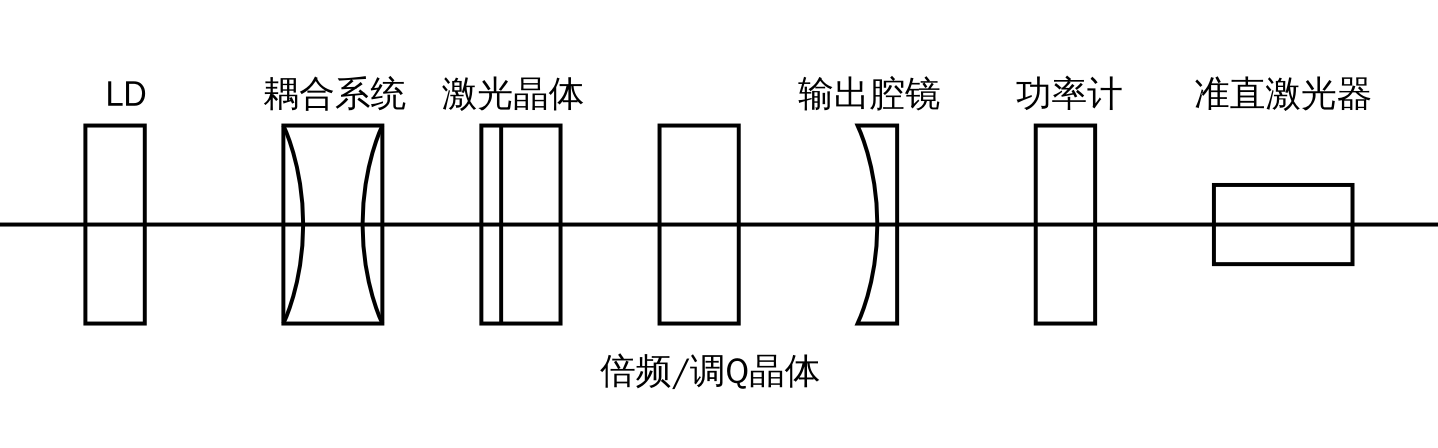
\includegraphics[width=0.7\textwidth]{pic1.png}
		\caption{\label{g:1}实验光路简图。实验装置如图所示,泵浦光源由半导体激光器产生808nm激光,由耦合系统将其偶合入激光晶体。激光晶体左侧渡有对于808nm透射对于1064nm反射的膜。激光晶体后面放入输出腔镜,形成激光光路,可以出射1064nm红外激光。功率计对激光进行测量,最右侧准直激光是辅助调整光路使用。调Q倍频晶体实在进行调Q或者倍频实验中才放入的,对激光腔内的激光进行一定的调整作用。}
	\end{center}
\end{figure}

這次实验使用的激光晶体Nd:YAG有着受激辐射截面大、光学质量好,热导率高等有点,而Nd:YVO$_4$晶体对于泵浦光源有着更好的吸收系数、更宽的吸收范围。两者都输出红外1064nm的激光。

实验中使用的调Q晶体是被动式的Cr$^{4+}$:YAG。其透过率会随着腔内的光强变化而变化,是一个非常典型的非线性光学晶体。随着泵浦的作用,腔内光子增加,调Q晶体的透过率也增加,达到饱和时透过率迅速增加,激光震荡形成发出激光,然后光子数目减少,透过率回复初始。这样形成了脉冲激光束。

而倍频晶体则是使用了KTP晶体。其极化强度矢量与入射场有明显的高阶项。当频率为$\omega$的光入射后会出现二级非线性效应,从而产生频率为$2\omega$的光波。本实验就使用此晶体倍频出现了频率为532nm的绿光。

\section{实验步骤以及数据}
\subsection{搭建固体激光器}
首先测量了半导体泵浦激光器的输出功率与输入电流之间的关系。如图\ref{g:2}所示组合光路图,调整泵浦电流的大小并测定输出功率,关系如图\ref{g:3}所示。

\begin{figure}[h]
	\begin{center}
		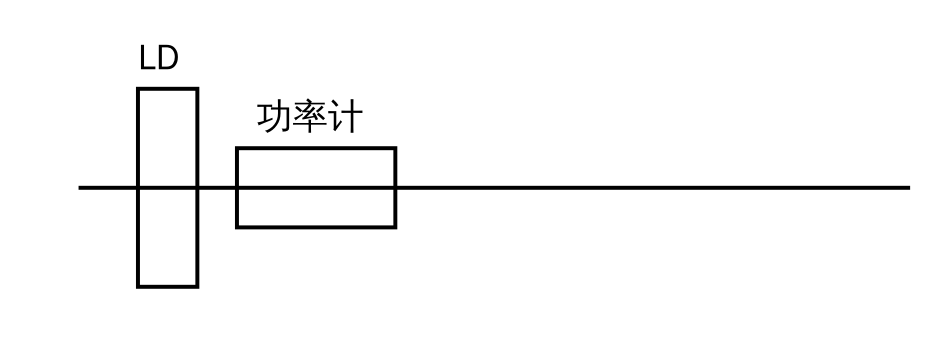
\includegraphics[width=0.7\textwidth]{pic2.png}
		\caption{\label{g:2}测量输入功率和电流的装置示意图。直接将功率计贴近泵浦光源测量即可。}
	\end{center}
\end{figure}
\begin{figure}[h]
	\begin{center}
		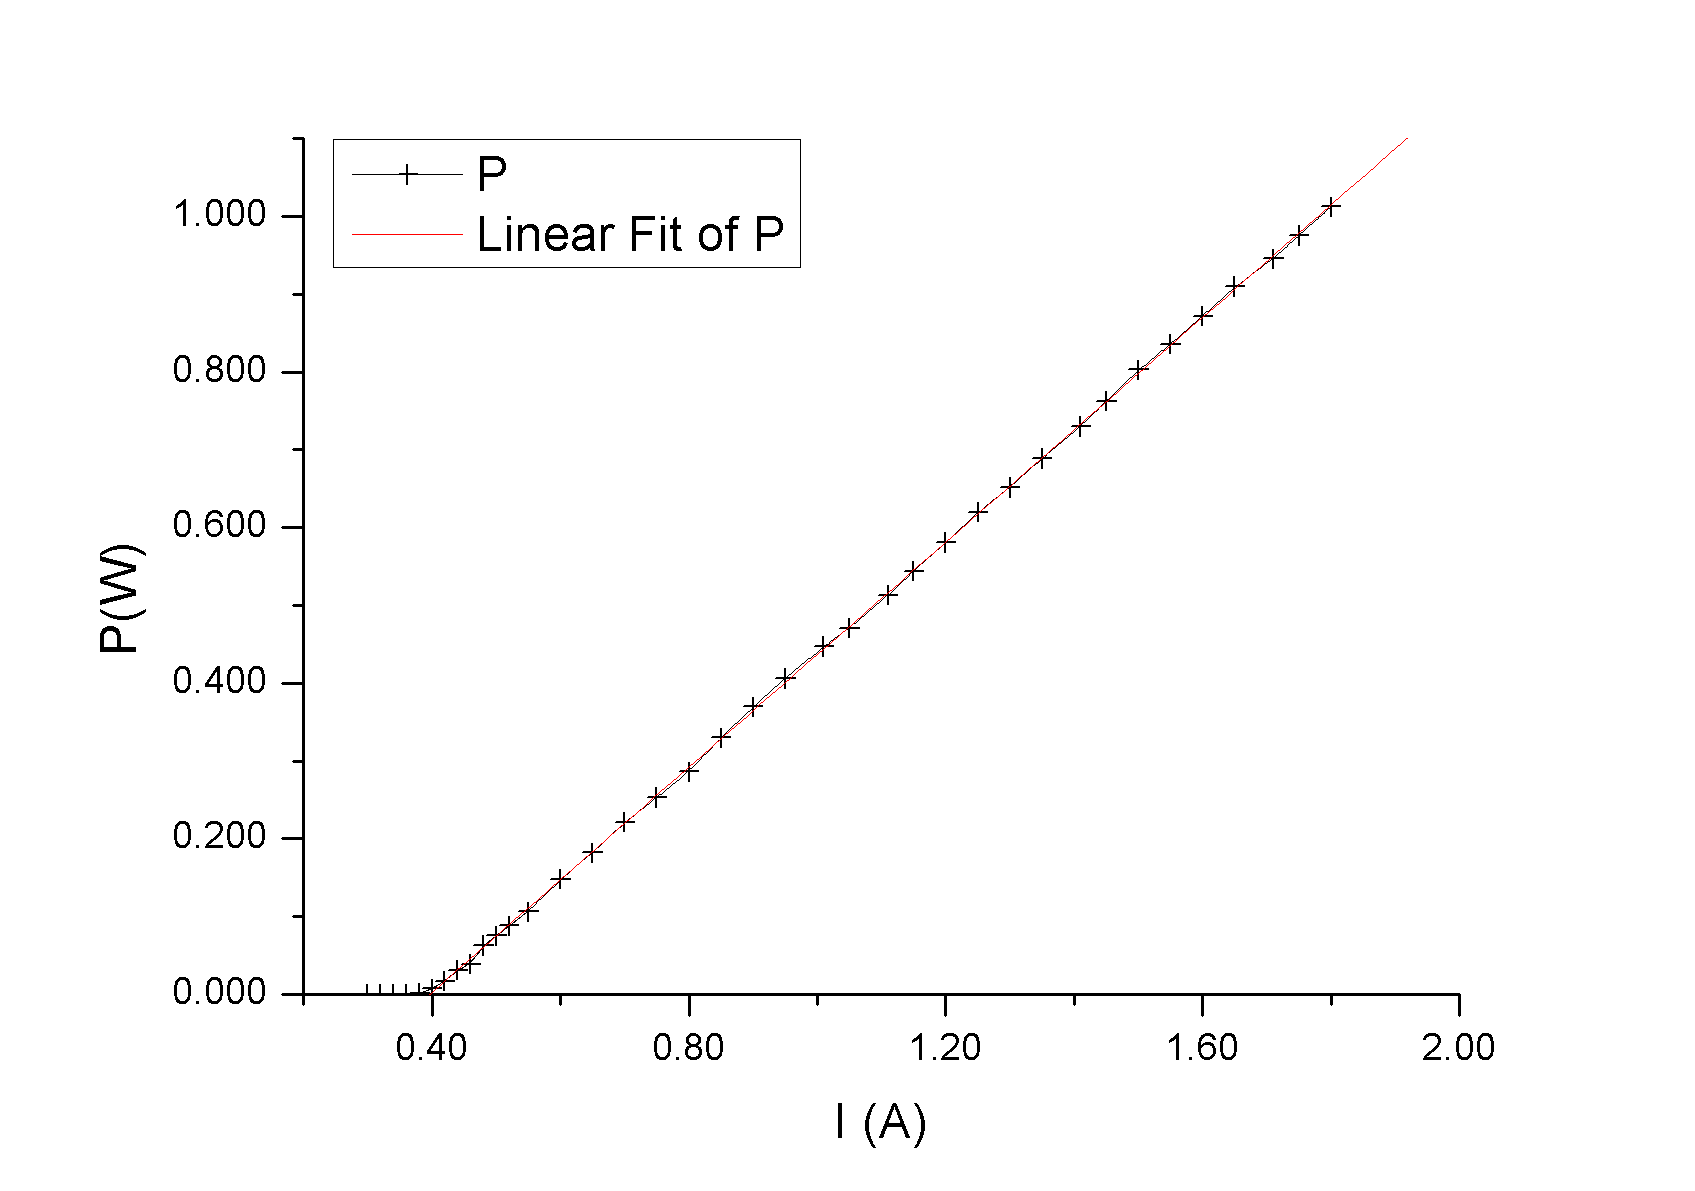
\includegraphics[width=0.7\textwidth]{pic3.png}
		\caption{\label{g:3}泵浦光功率和泵浦电流大小之间的关系图。可以看出在达到半导体的阈值电流之后,光功率和电流成非常好的线性关系。其中拟合的区域是超过阈值电流后的数据点的拟合。}
	\end{center}
\end{figure}

从泵浦电流大小和输出功率之间的关系可以看出,半导体激光器的阈值电流为0.38A。当泵浦电流超过这个电流后输出功率和电流有着良好的线性关系。

随后搭建激光器,如图\ref{g:4},将泵浦光源,耦合透镜,激光晶体和输出腔镜放入光路,利用准之激光使之之间近似准直。然后细致调节输出腔镜和激光晶体,使得两者之间的达到平行,输出的激光功率最大。这时候可以测量到红外激光器的输出功率和泵浦电流之间的关系。记录两种激光晶体的输出功率,如图\ref{g:5}所示。

\begin{figure}[h]
	\begin{center}
		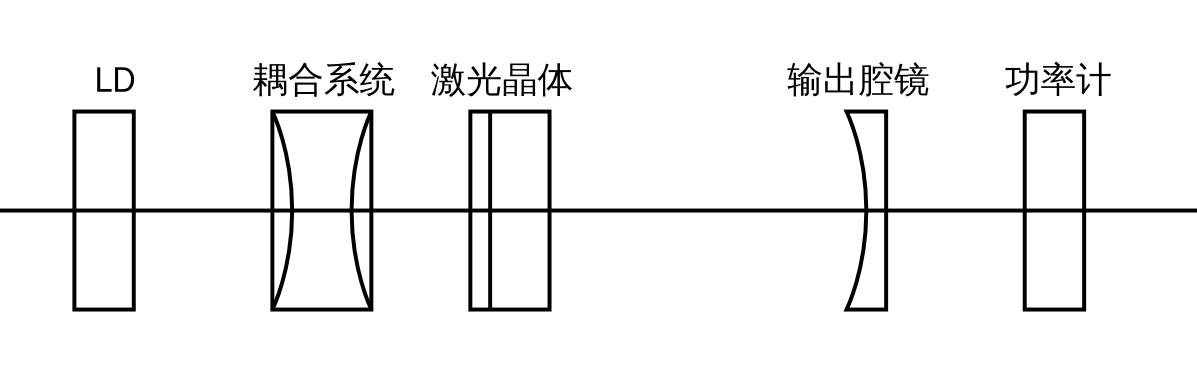
\includegraphics[width=0.7\textwidth]{pic4.png}
		\caption{\label{g:4}激光器示意图。激光在激光晶体和输出腔镜之间形成,输出腔镜透射率为3\%。}
	\end{center}
\end{figure}
\begin{figure}[h]
	\begin{center}
		\subfigure[激光输出功率和泵浦电流之间的关系]{
		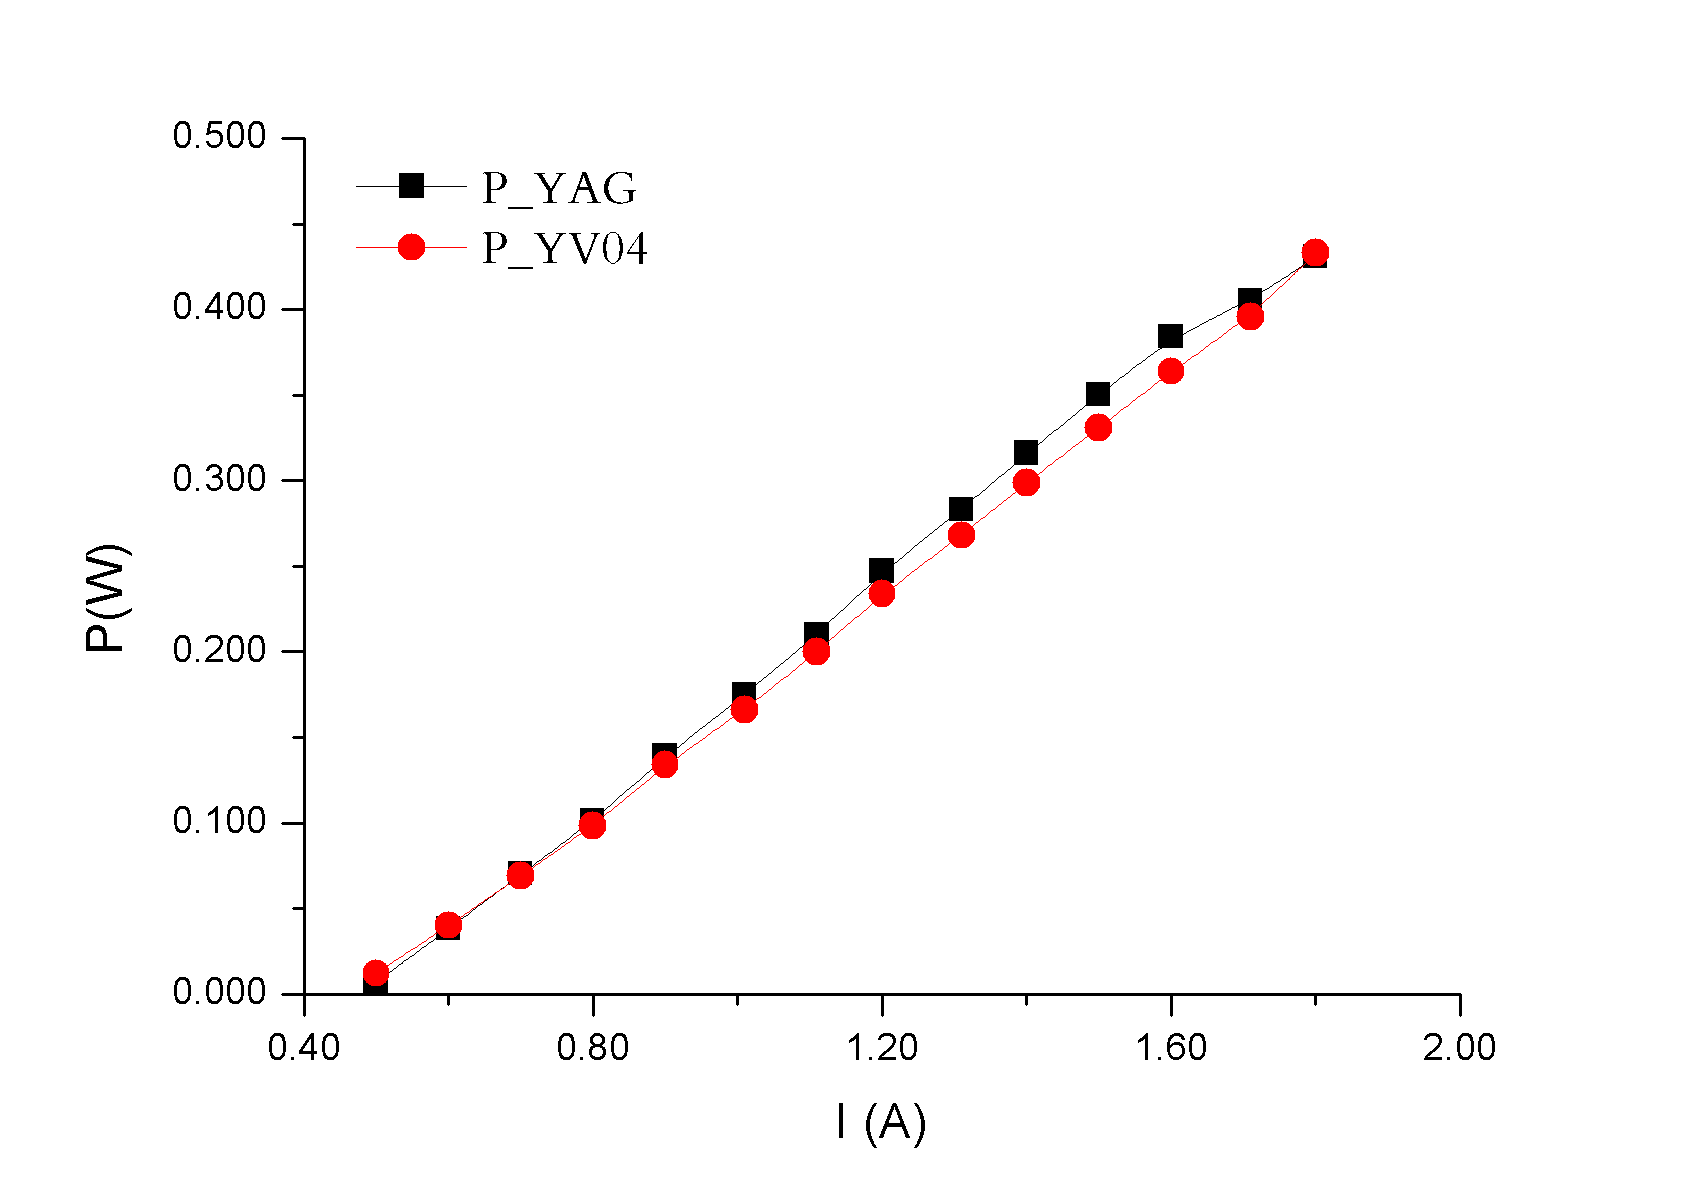
\includegraphics[width=0.7\textwidth]{pic5.png}
	}
	\subfigure[激光转换效率和泵浦电流之间的关系]{
		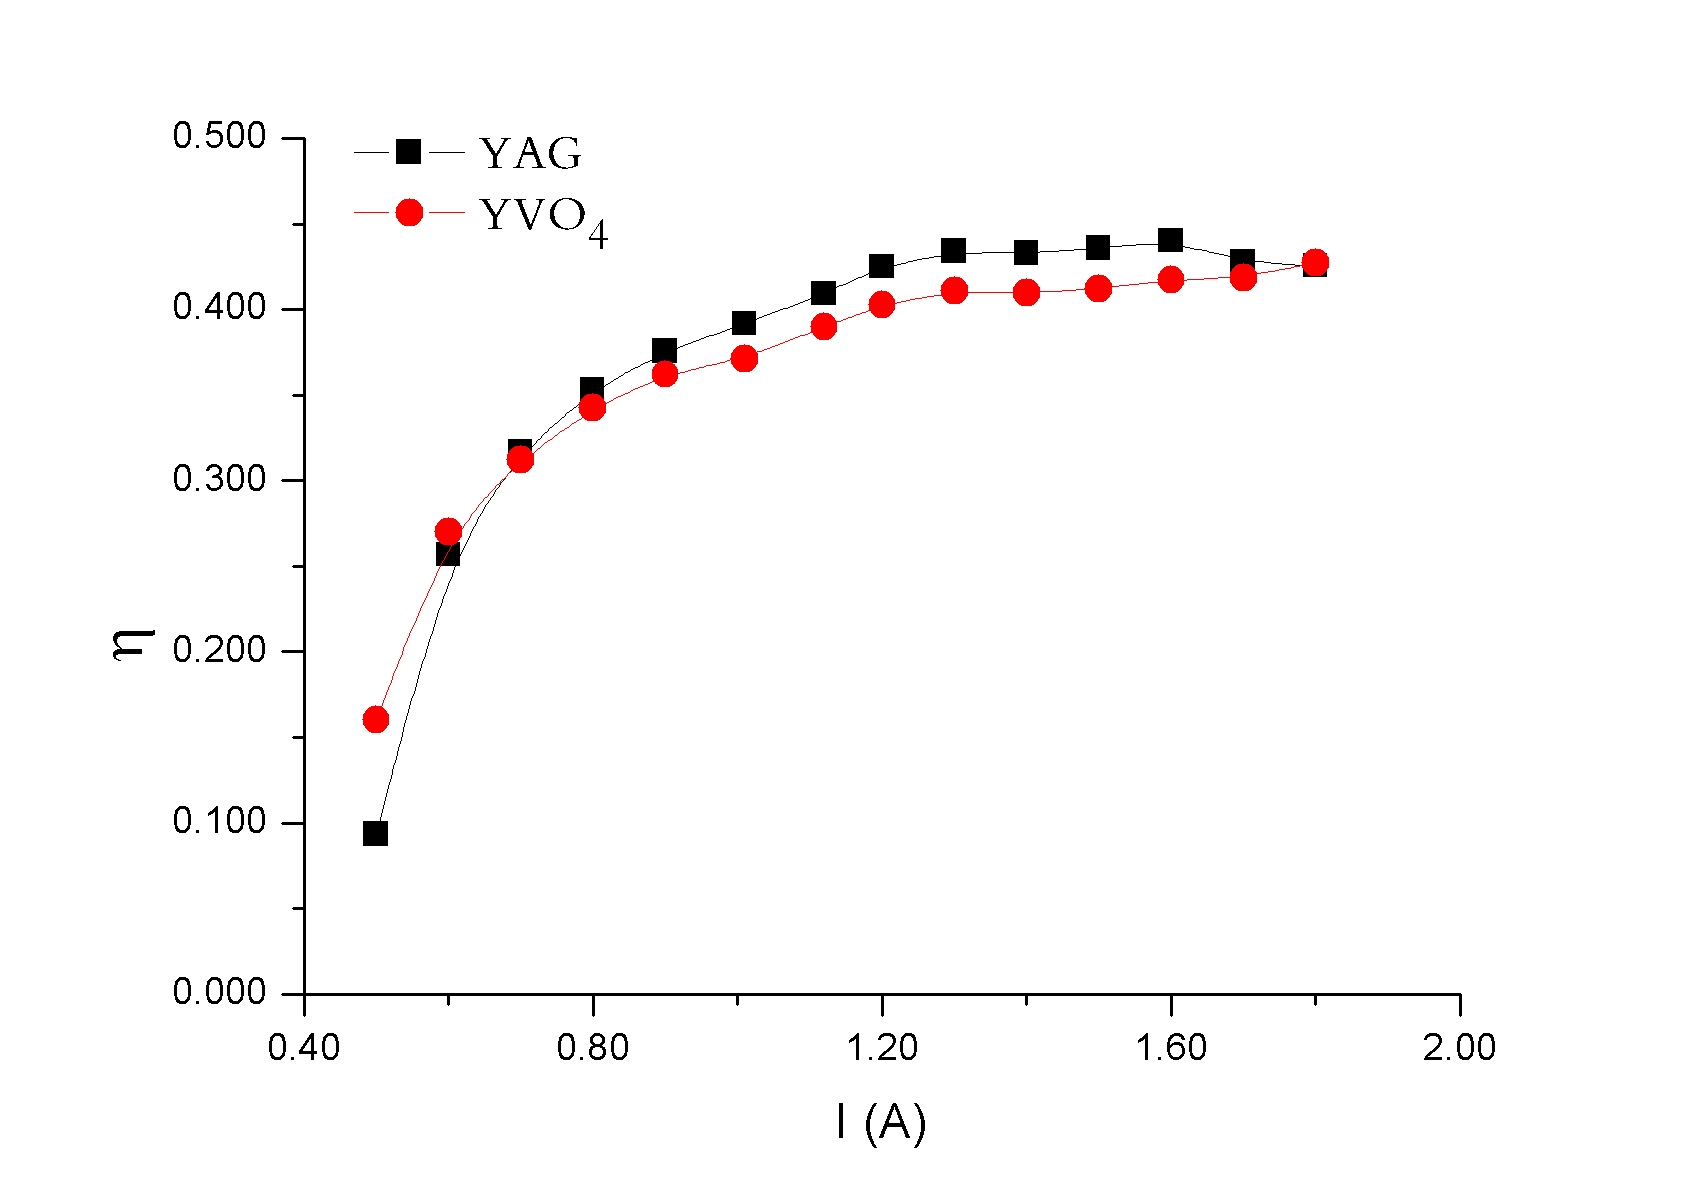
\includegraphics[width=0.7\textwidth]{pic6.png}
	}
		\caption{\label{g:5}激光器输出功率和泵浦电流之间的关系图。红色为YVO$_4$晶体,黑色为YAG晶体。两者的阈值电流基本上就是0.4A。输出功率关于泵浦电流基本上是线性关系,转换功率最后约稳定在40\%左右}
	\end{center}
\end{figure}

从测量的图可以看出,晶体Nd:YAG和晶体Nd:YVO$_4$的效率基本一致。这一点并不是十分的合理,我觉得可能的原因是因为调整YVO$_4$的时候调整的可能有一些偏移,同时耦合透镜可能耦合的效率不是特别的高以至于本身输入晶体的能量就有一定的损失。对图片分析可以看出,激光器输出的功率和输入的泵浦电流基本上成线性关系(在电流超过阈值的时候)。两者转换效率最后也基本稳定在40\%左右,这可以认为为饱和转换效率。
\subsection{被动调Q产生激光脉冲}

产生脉冲激光是在YVO$_4$晶体和输出腔镜之间加入了一个Cr$^{4+}$YAG调Q晶体,使其输入了脉冲激光。调整调Q晶体,激光晶体以及输出腔镜使得输出激光的平均功率最大。然后将其输入到功率探测器,测量其平均功率,同时用快速探测器链接示波器以探测其脉冲宽度,周期的关系。可以得到如下\ref{t:1}的数据
\begin{center}
	\begin{table}
		\caption{被动调Q激光脉冲平均功率,重复频率,脉冲宽度和泵浦电流的关系表}
		\label{t:1}
		\begin{tabular}{m{3cm}<{\centering}m{3cm}<{\centering}m{3cm}<{\centering}m{3cm}<{\centering}m{3cm}}

			\hline
			\hline
			I/A&P$_{out}$&f/Hz&$\Delta t/\mu s$\\
			\hline
			1.8&0.038&78&0.3\\
			1.6&0.026&61&0.3\\
			1.4&0.018&42&0.3\\
			1.2&0.012&56&0.4\\
			1.0&0.005&46&0.3\\
			0.8&0.001&-&-\\
			\hline
		\end{tabular}
	\end{table}
\end{center}

从表中可以看出来,随着泵浦电流的逐渐增大,平均输出功率也在变大,相应的频率有增大的趋势,而泵浦的脉冲宽度基本没有太大的变化,这一点我们认为将腔内功率输出所消耗的时间和腔内光强是没有太大的关系的。而调Q晶体达到阈值的速度则和腔内的功率有关系。所以频率增高,而脉宽基本没有太大的变化。

\subsection{KTP晶体二倍频实验}

将上实验中的调Q晶体替换为KTP晶体,并将输出透镜更换为透射率为1\%的透镜,细致的调整光路的准直,这时候就应该能够看到明显的绿光,这是532nm的绿光,也就是1064nm红外激光倍频而来的。调节KTP晶体的光轴的方向可以看到绿光光斑的明亮随着角度而变化,这一点是因为KTP晶体光轴改变从而改变了相位匹配的程度,影响到了倍频的转换效率。

改变泵浦电流的大小可以测量的道输出功率随着泵浦电流的改变的数据。数据图如\ref{f:6}

\begin{figure}[h]
	\begin{center}
		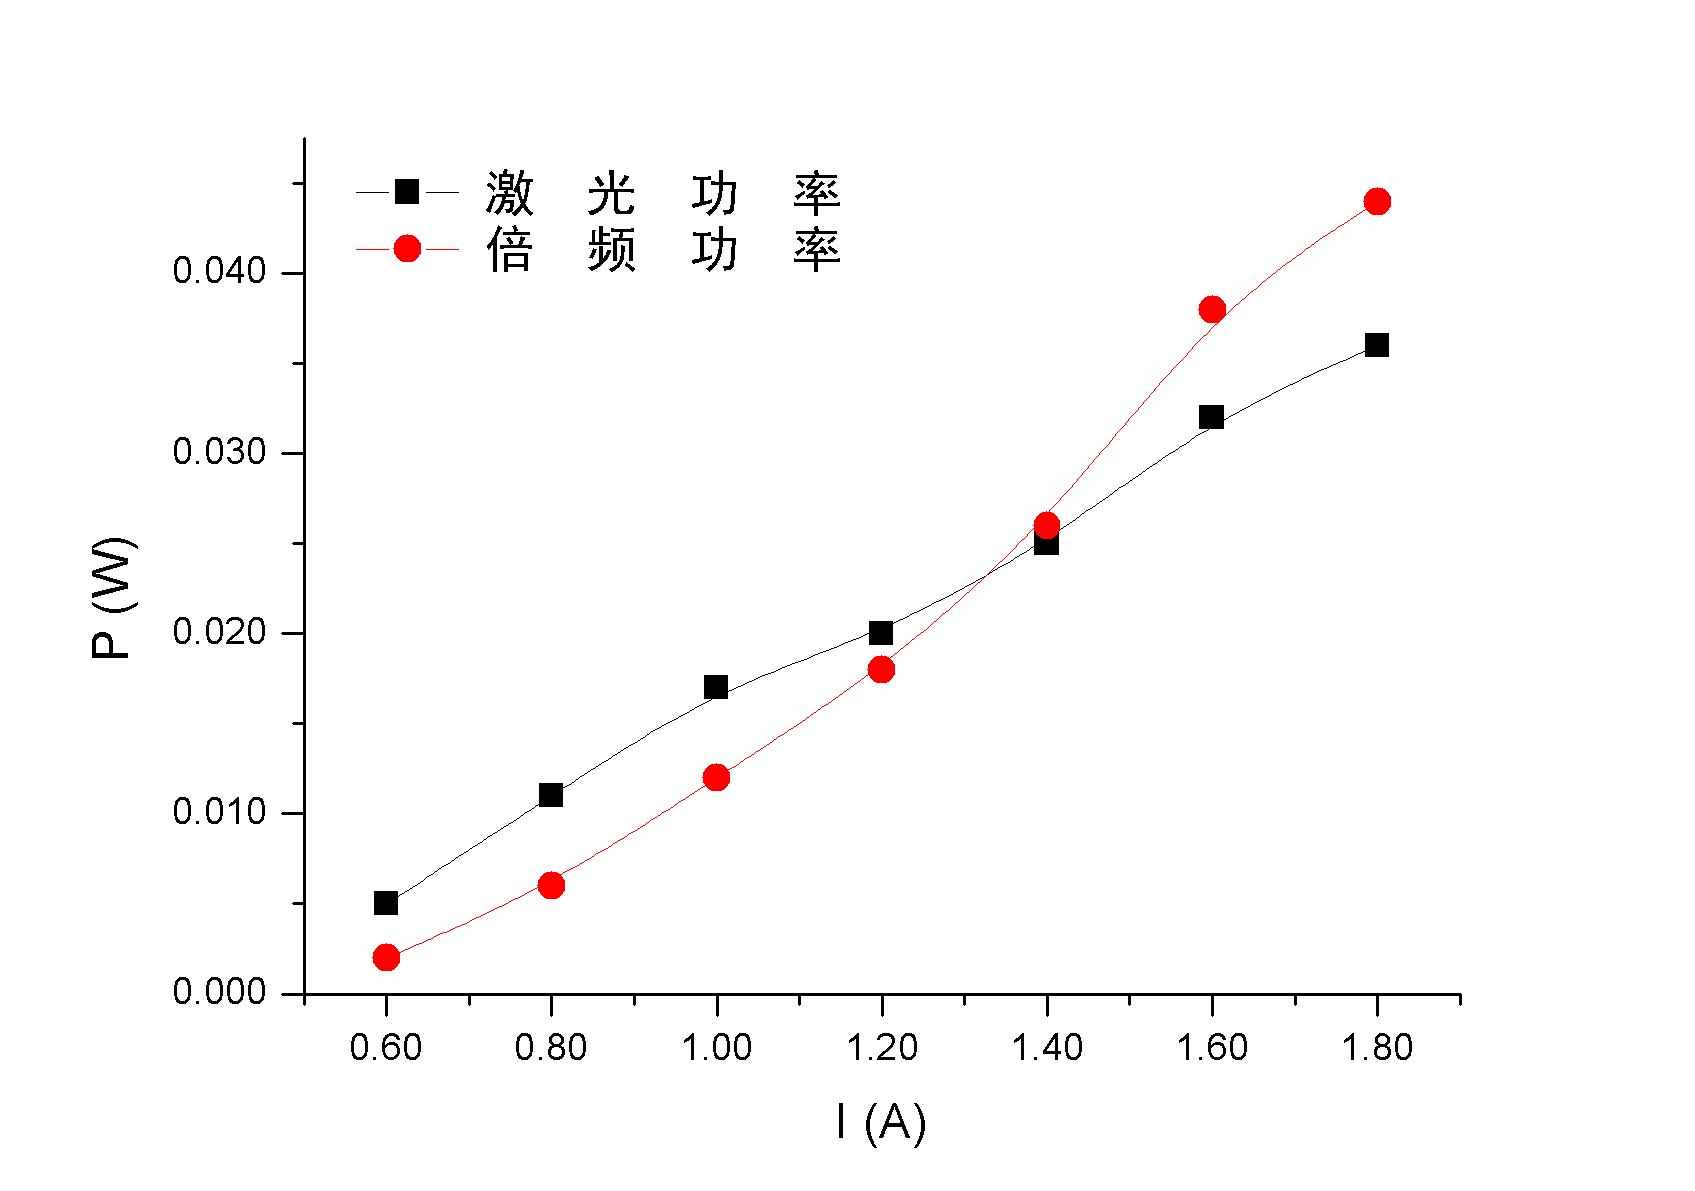
\includegraphics[width=0.7\textwidth]{pic7.png}
		\caption{\label{g:4}二倍频实验输出功率和泵浦电流关系图。如图所示,黑线为未经过倍频,直接采用1\%输出透镜测量到的激光功率和泵浦电流之间的关系。红线则是经过KTP晶体二倍频之后的输出功率和泵浦电流之间的关系。可以看出倍频后的转换效率更高一些。}
	\end{center}
\end{figure}

这里可以看出经过倍频后输出的激光功率更高,这里我认为是对于1\%的透镜而言,频率532nm的绿光在这个腔体内的转换效率要高于1064nm的激光,从而测量得到相对饱和的时候倍频后的激光转换效率是高于没有倍频的效率的。


\section{结论}
本实验利用半导体激光器作为泵浦光源,使用Nd:YAG和Nd:YVO$_4$两种激光晶体产生红外激光。其中半导体激光器的输出功率和泵浦电流在超过阈值电流0.4A后基本成线性关系,而激光晶体产生的激光在0.4A后也基本成线性关系。两个晶体的转换效率最大在40\%~45\%左右。插入调Q晶体后可以输出激光脉冲,其频率随着泵浦电流的增大而增大,脉冲宽度基本上是稳定的0.3$\mu s$。加入KTP晶体则可以观察到倍频效应,出现了明显的绿色激光。其功率随着泵浦电流的增加而增加。

\section{致谢} 
感谢蒋莹莹老师的指导,以及贾春燕,冉书能老师的技术支持。


\begin{thebibliography}{}
	\bibitem{Book} 吴思成,王祖铨~2010 近代物理实验(第三版)(北京:高等教育出版社)第154页.%
%
\end{thebibliography}

\clearpage
\appendix
\section{记录本}
\begin{figure}[h]
	\begin{center}
		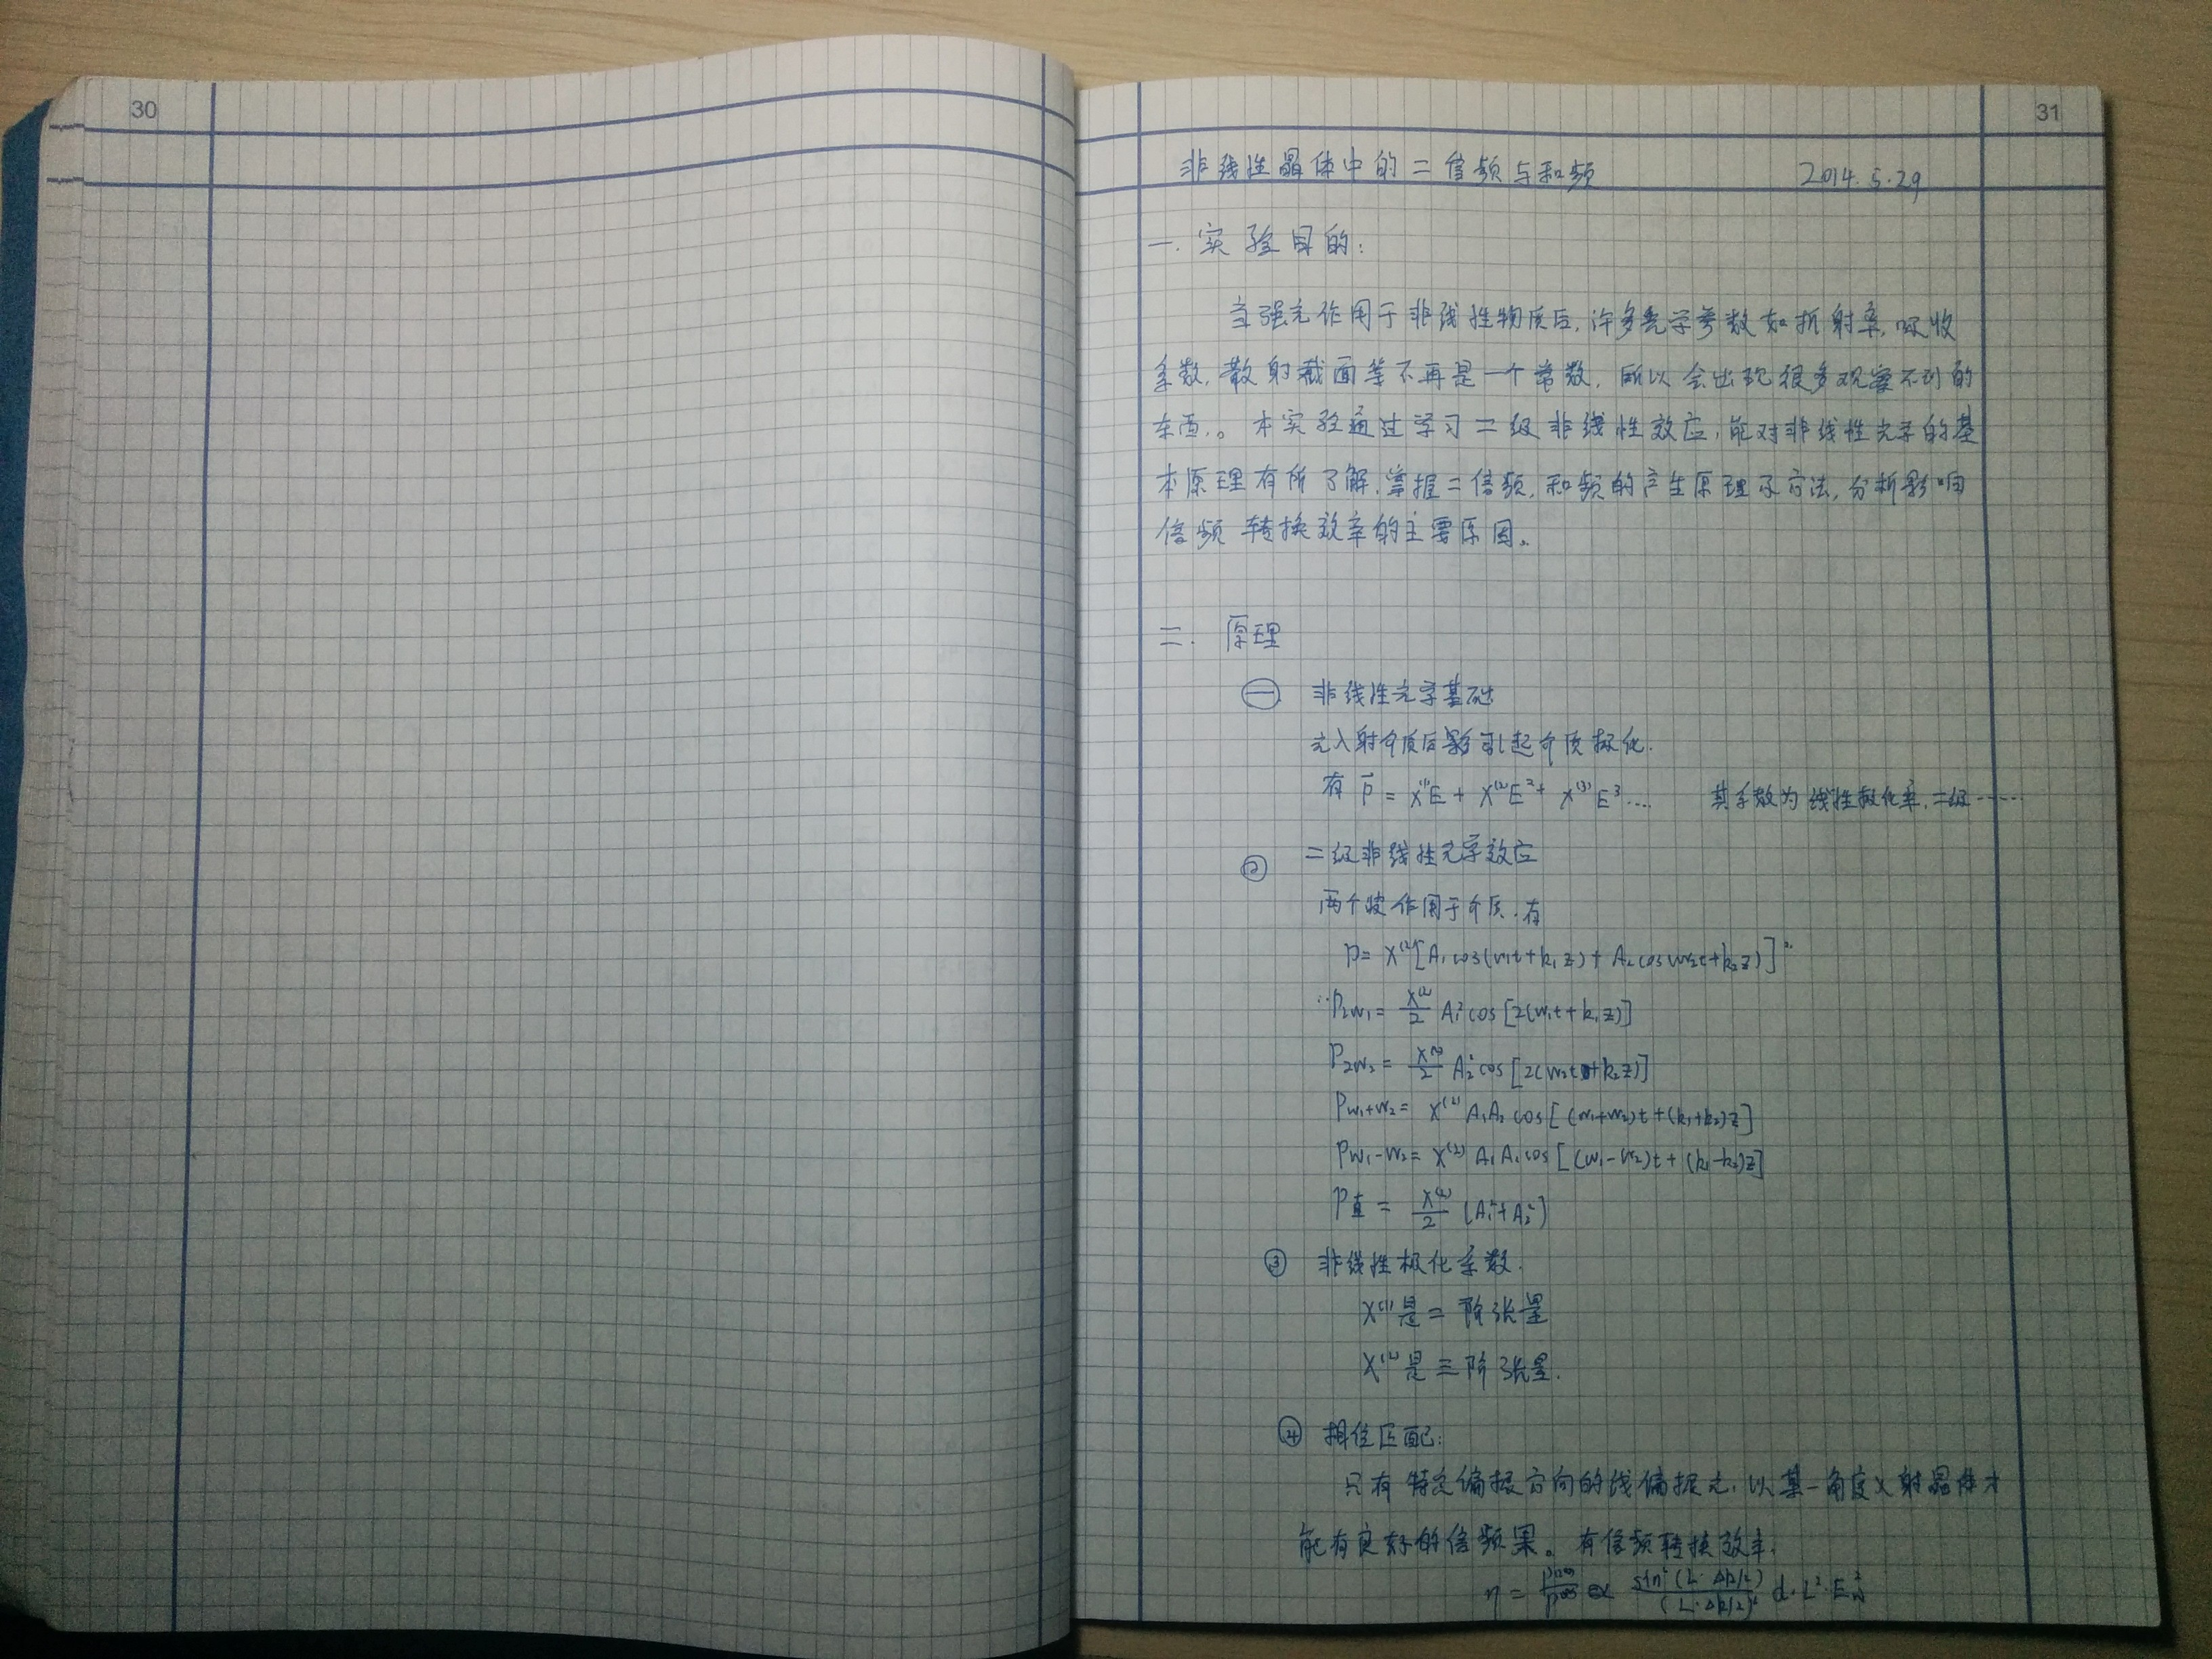
\includegraphics[width=0.7\textwidth]{pic8.jpg}
	\end{center}
\end{figure}
\begin{figure}[h]
	\begin{center}
		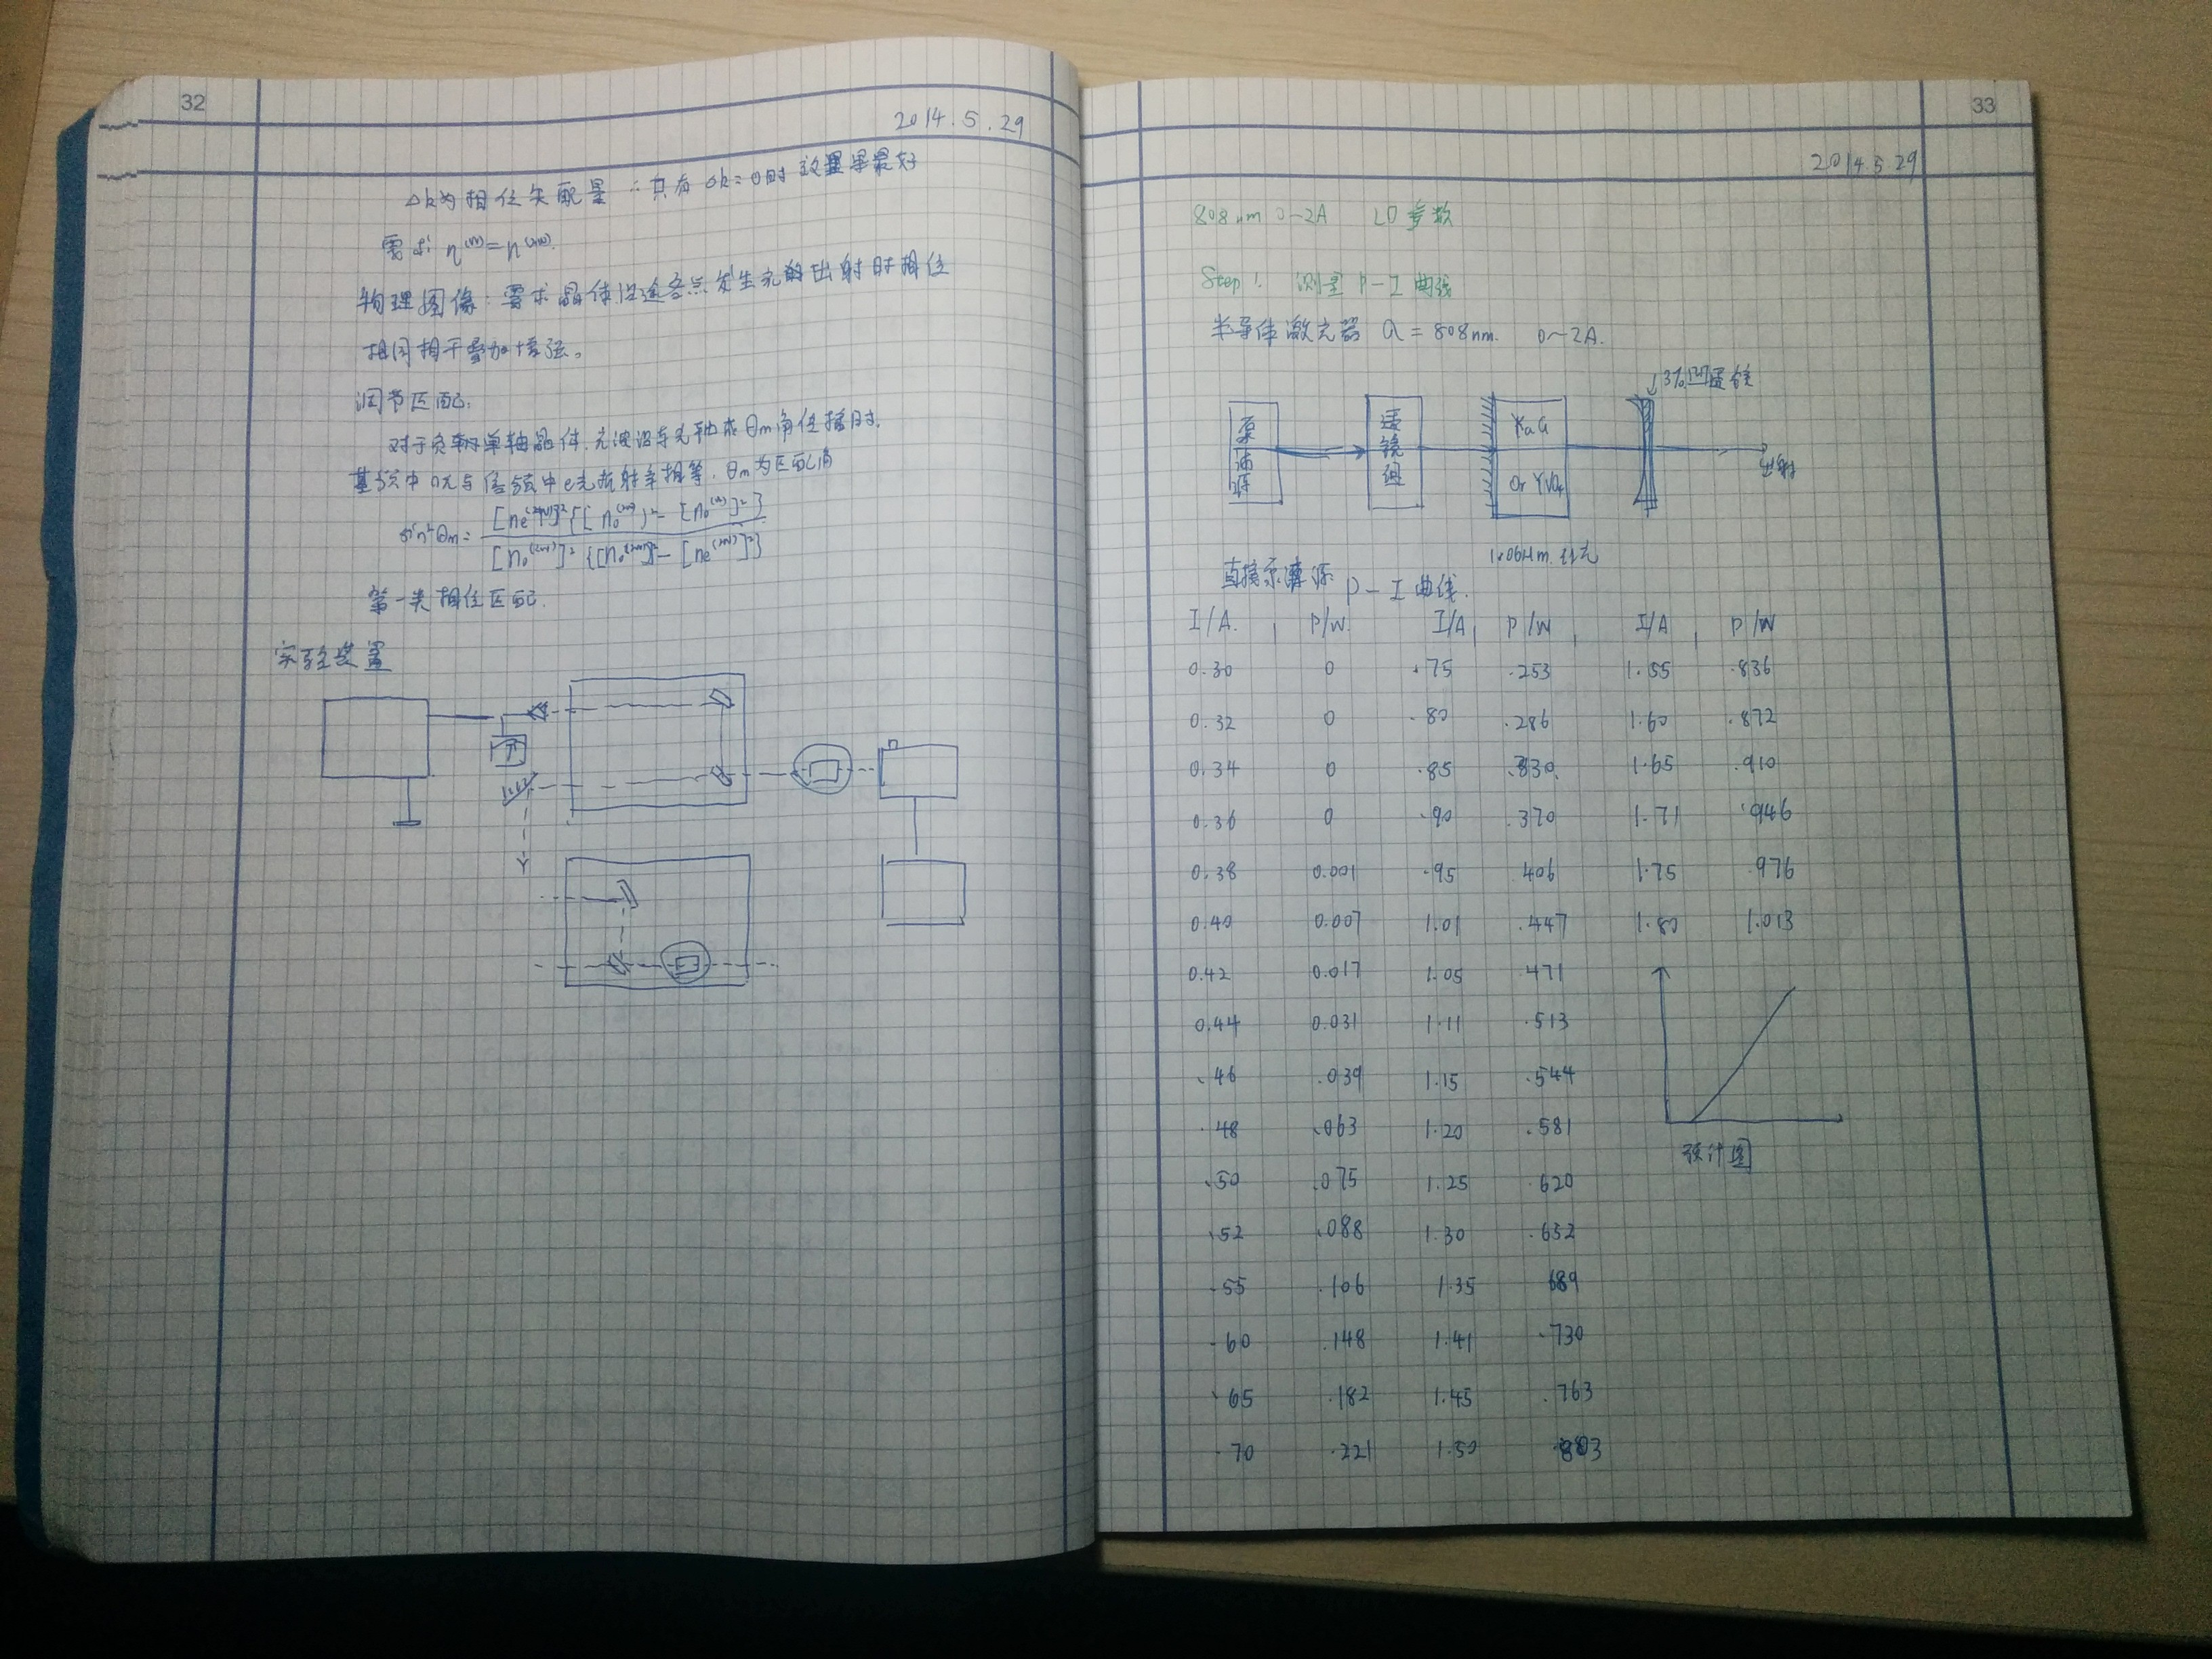
\includegraphics[width=0.7\textwidth]{pic9.jpg}
	\end{center}
\end{figure}
\begin{figure}[h]
	\begin{center}
		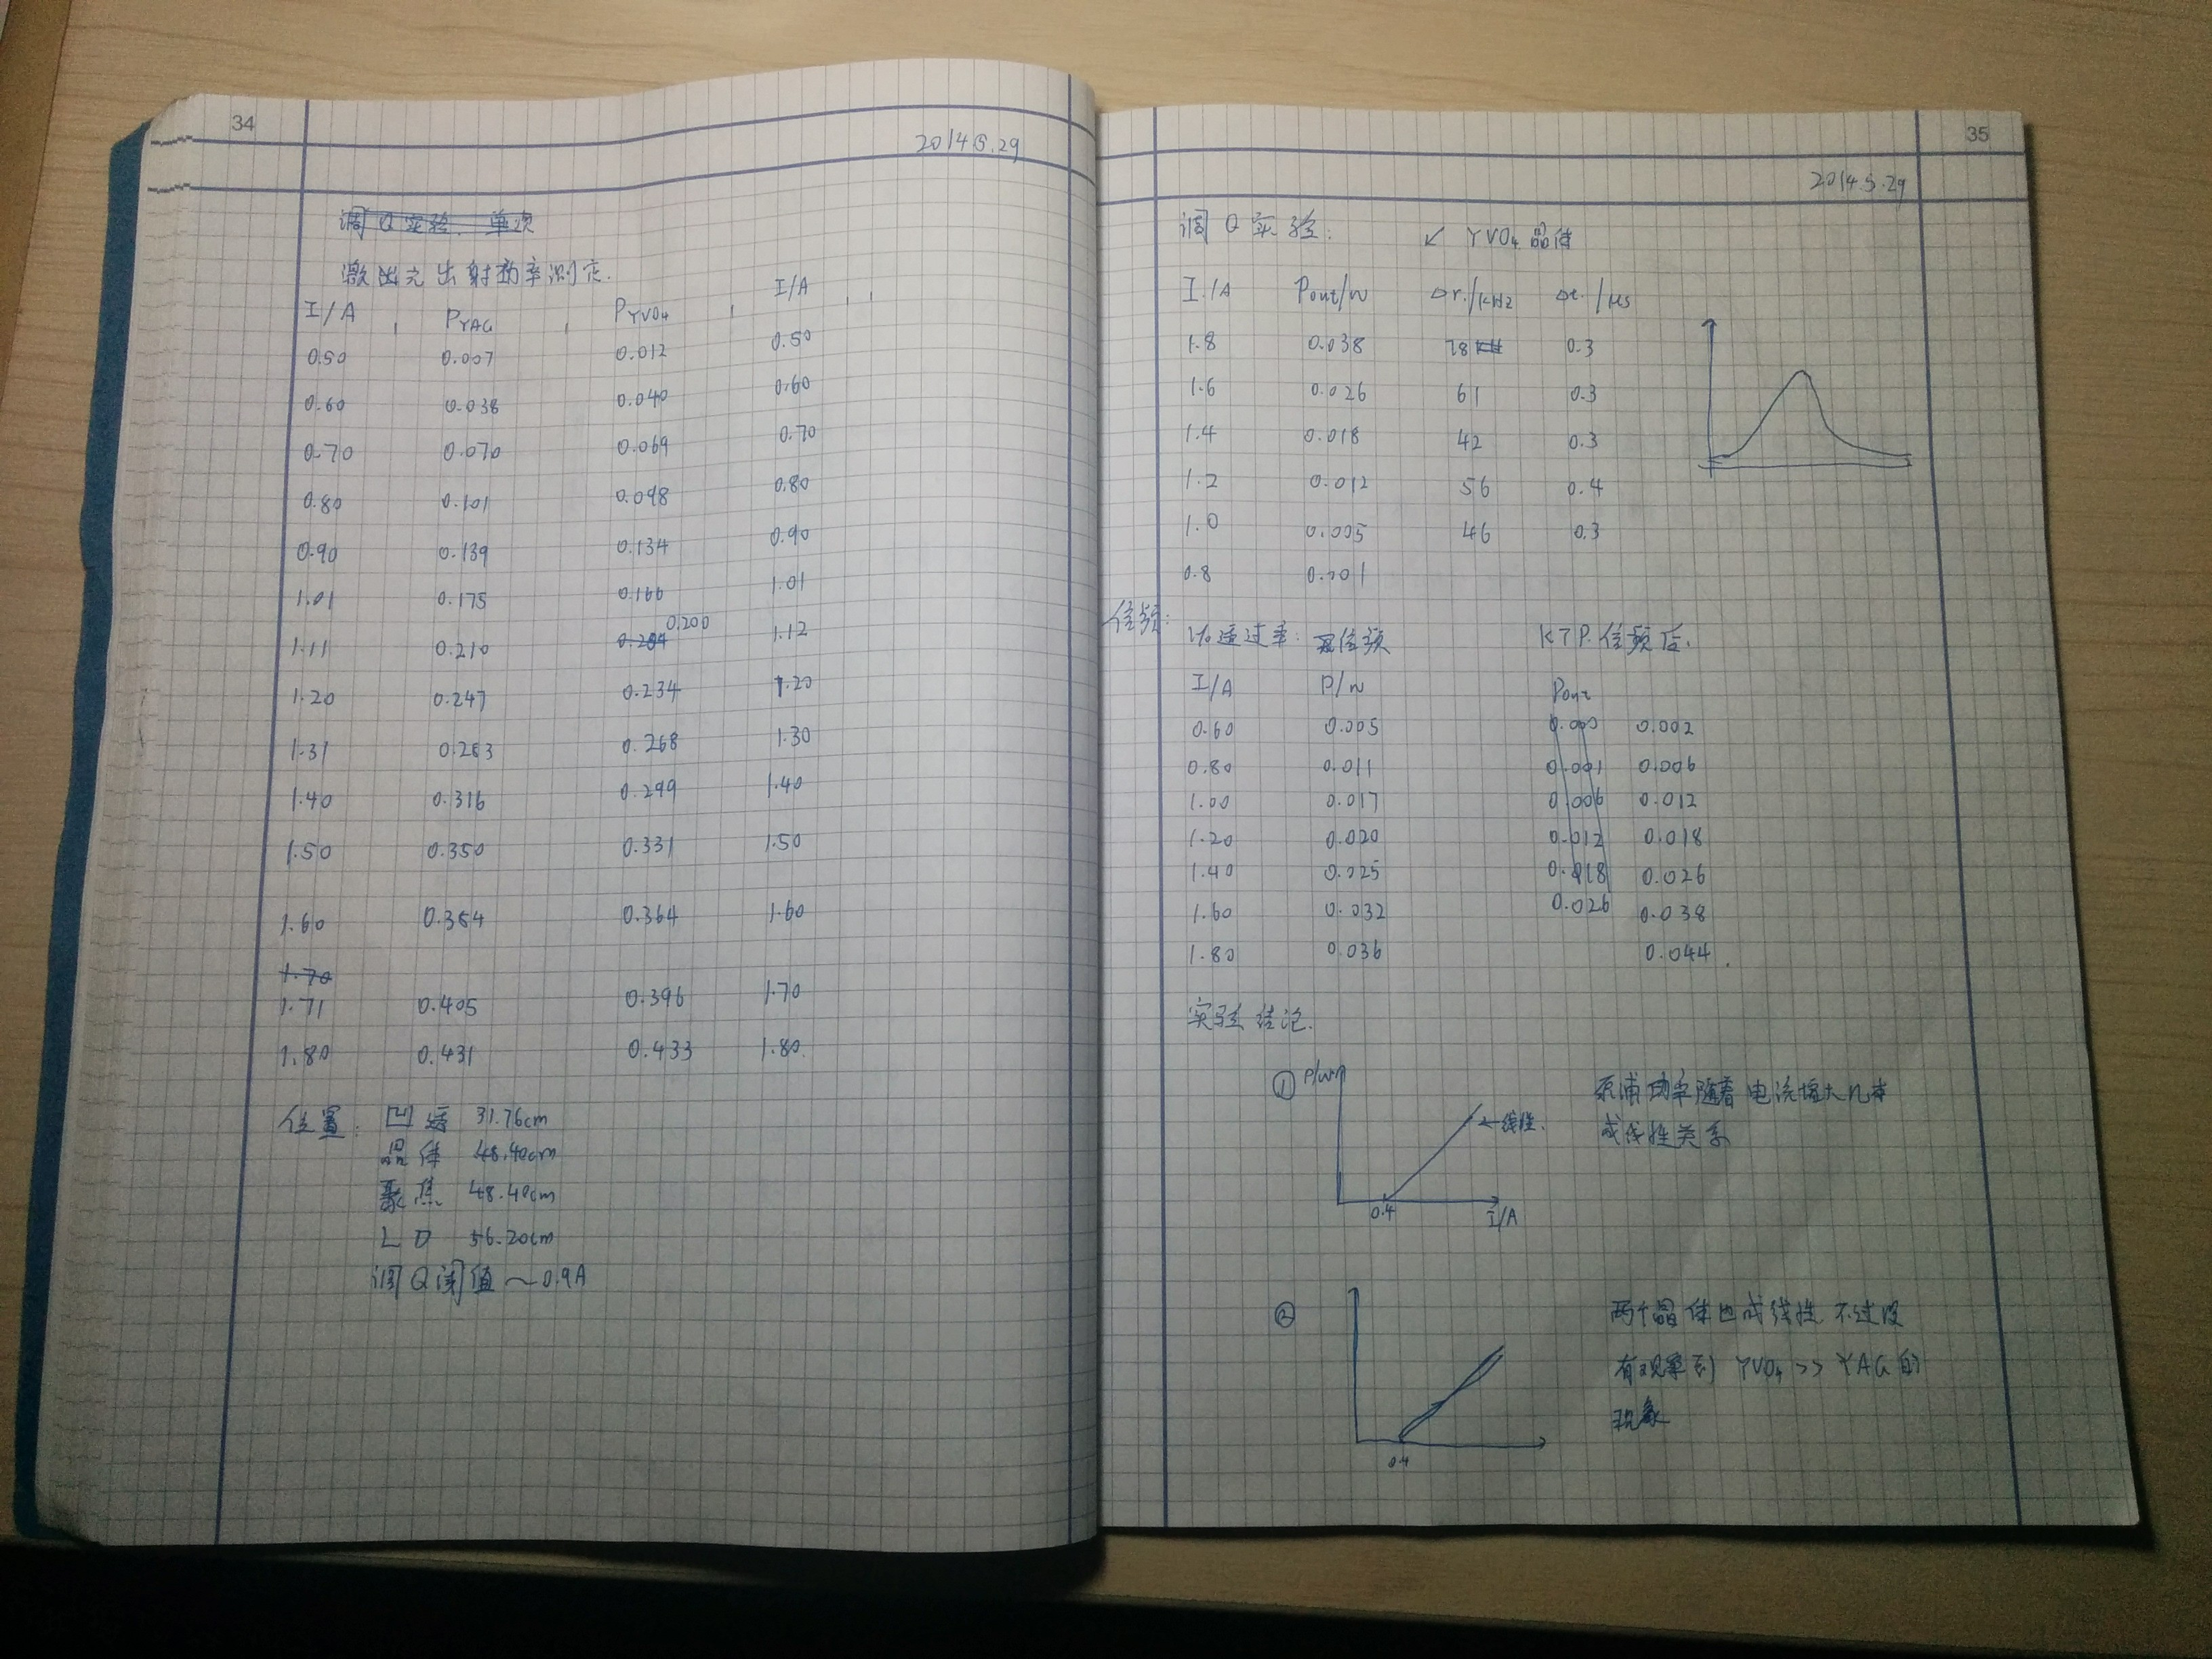
\includegraphics[width=0.7\textwidth]{pic10.jpg}
	\end{center}
\end{figure}
\begin{figure}[h]
	\begin{center}
		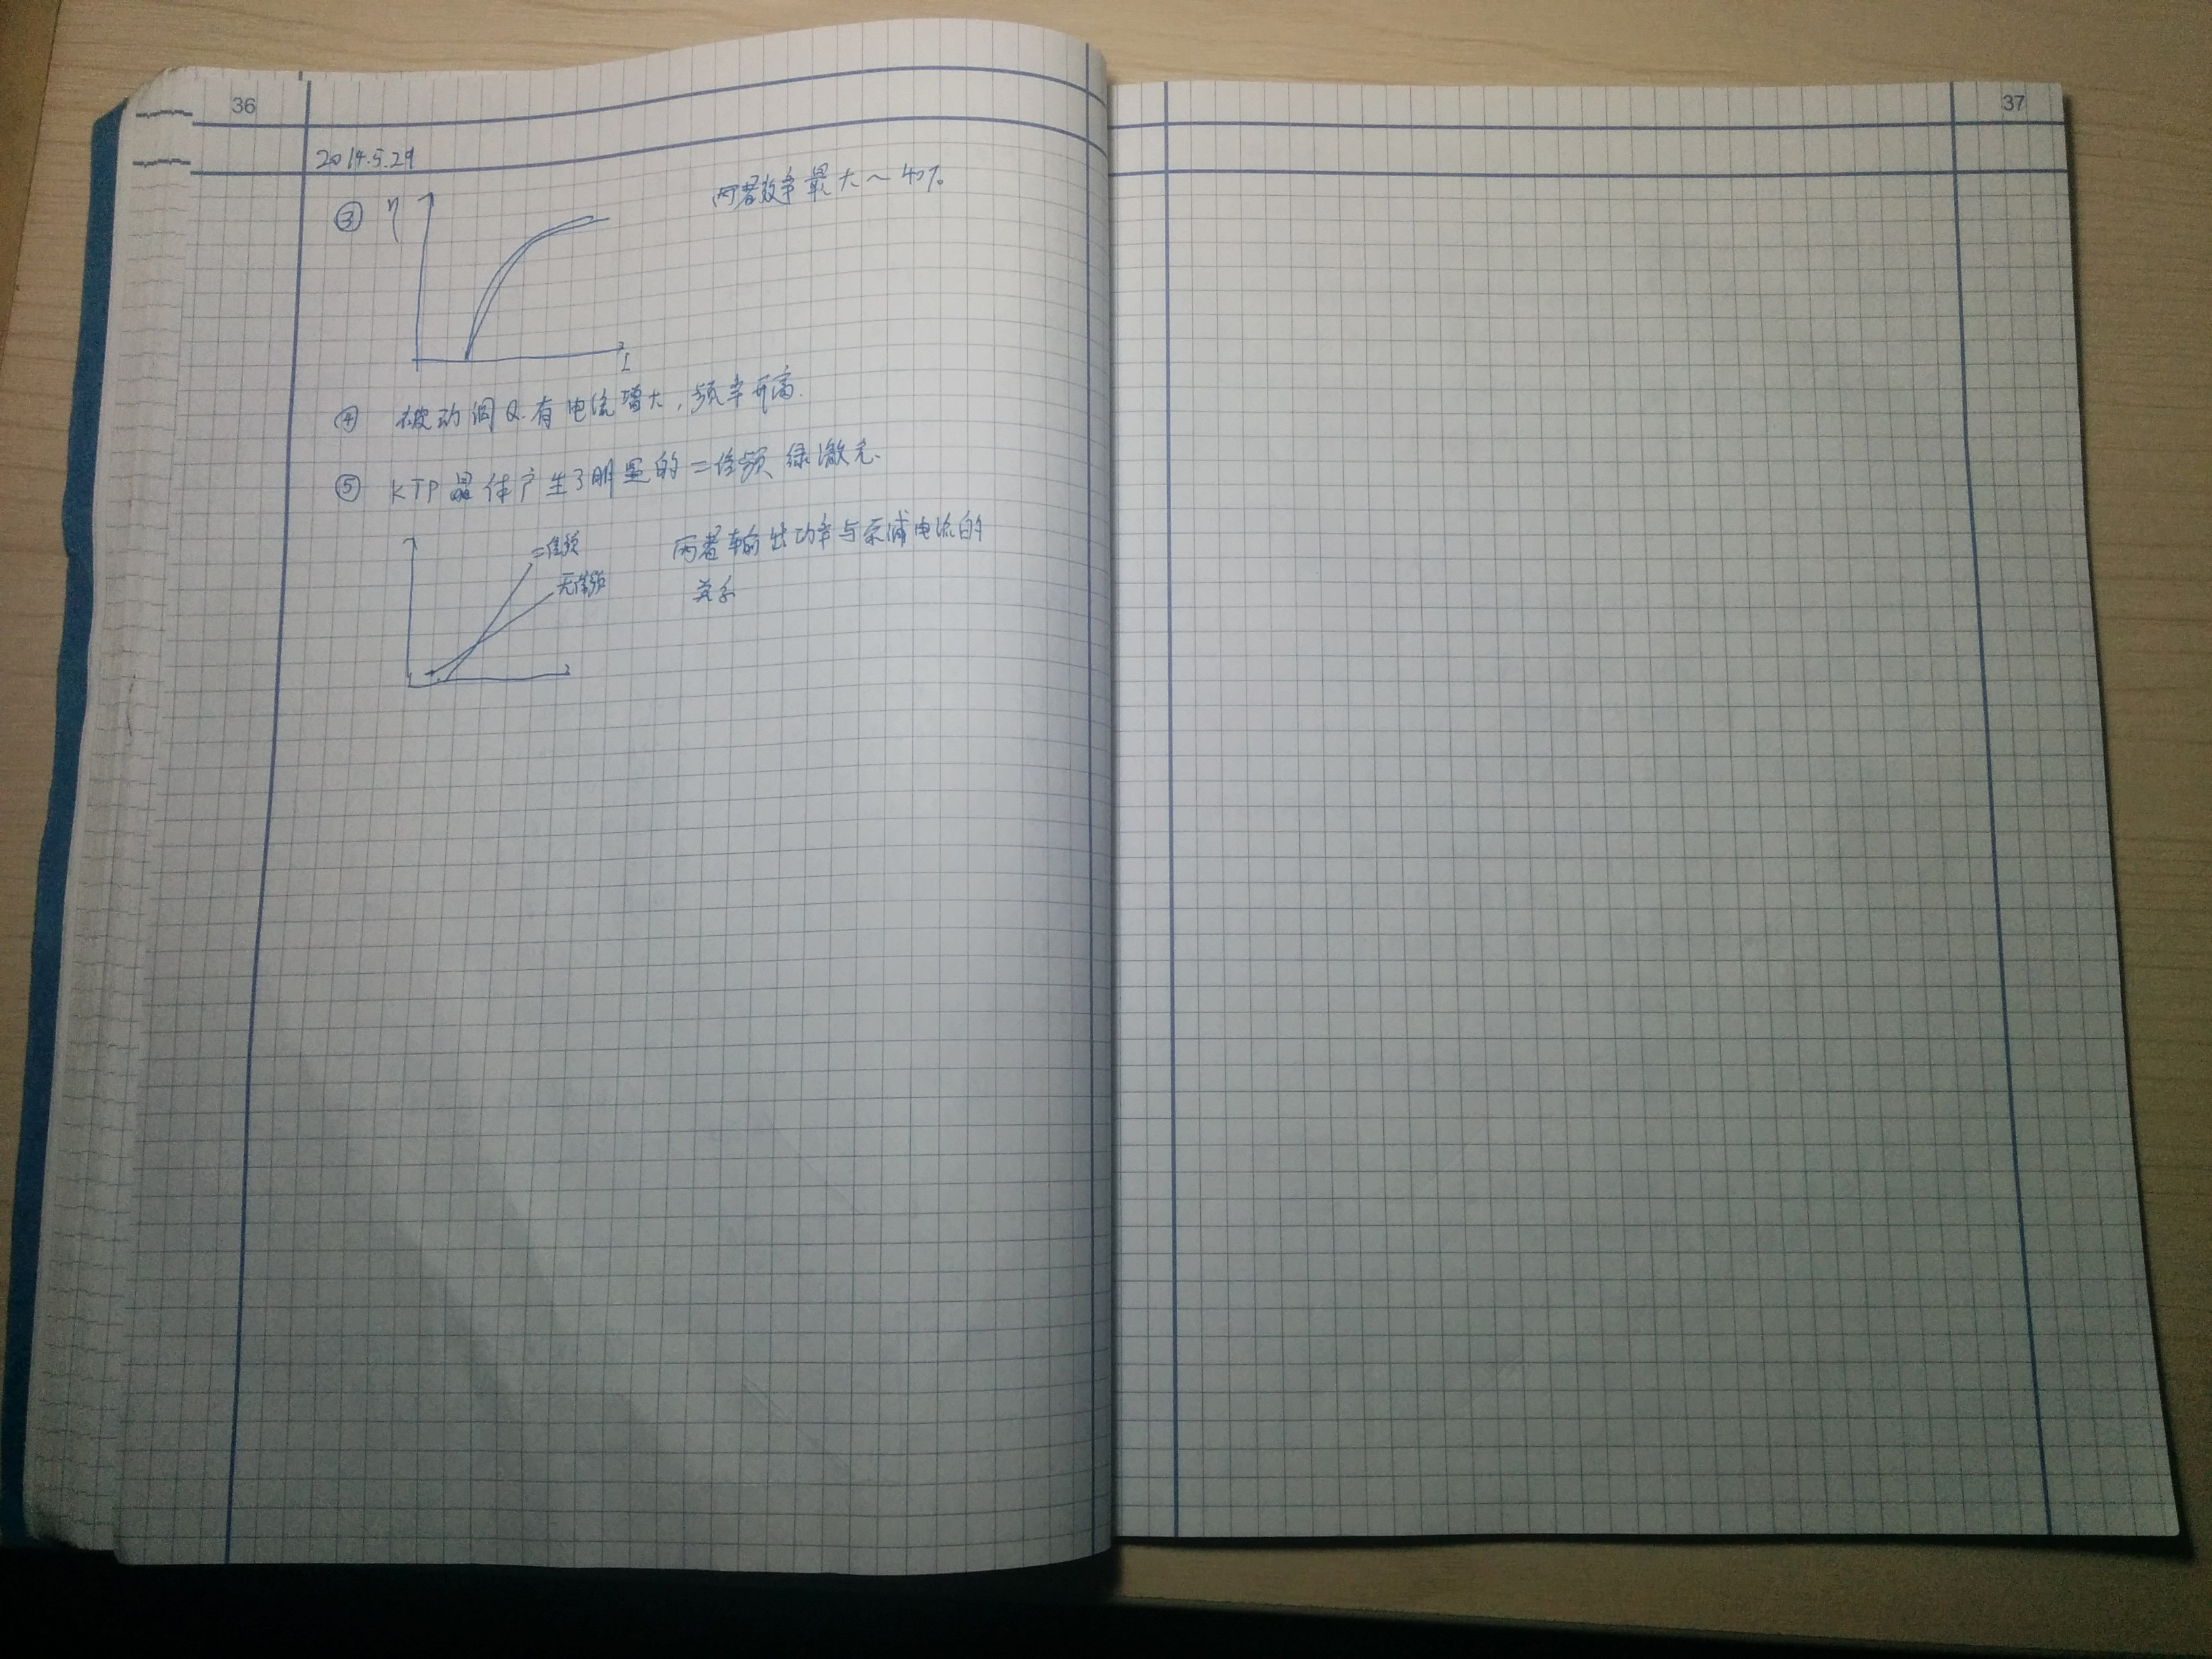
\includegraphics[width=0.7\textwidth]{pic11.jpg}
	\end{center}
\end{figure}
\end{document} 
